\section{Divergence Point Example}
This example shows a simple \emph{toy model} of some cognitive process that is able to produce a
so called \emph{divergence point} \cite{Reingold2012}. A divergence point of two response latency
distributions is the earliest time point at which the two response latencies differ. Obviously, 
there can't be any divergence point if the two response latency distributions are analytic 
(e.g., the convolution (chain) of Gamma distributions, \cite{Gelooven1999}). This example, however,
not only shows how a non-analytic response-latency distribution may arise that allows for a 
divergence point, but has an actual divergence point%
\footnote{One distribution being non-analytic is a necessary but not a sufficient condition.}. 

This very simple model consists of 3 $\Gamma$-distributed random variables $C, X_1$ and $X_2$,
where the latter is a shifted Gamma distribution (here shifted by $300$ ms, i.e. 
$X_3 \sim \Gamma(T-300; k, \theta)$).  The model is
\begin{align}
 \text{control: } & R_c = C + X_1 & \text{ where } C \sim \Gamma(c; 3, 20),\,X_1\sim\Gamma(x_1; 10,30)\\
 \text{experimental: } & R_e = C + \min(X_1, X_2) & \text{ where } X_2 \sim\Gamma(x_2-300; 1, 70)\,.
\end{align}

This model can be read as: Under control condition, the stimulus triggers a common stage $C$ which then 
triggers a second stage $X_2$ that itself immediately triggers the response. Under experimental condition,
again the stimulus triggers the common stage $C$ which then triggers $X_1$. Additionally, the common
stage $C$ also triggers the delayed stage $X_2$ in parallel to $X_1$. The response is then triggered by 
either $X_1$ or $X_2$, depending on which stage completes first. Consequently, the response latency
under control condition is $R_e = C + \min(X_1,X_2)$.

The following code shows how this simple model is implemented using the Python API of StochBB.

\begin{lstlisting}[language=Python]
from numpy import *
import stochbb;

# Processing model
d = 300
C = stochbb.gamma(3,20)
X1 = stochbb.gamma(10,30)
# shifted exponential
X2 = stochbb.gamma(1,70) + d

# response latency control condition
#   is simply R = C + X1
Rc = C + X1
# and for the experimental condition
Re = C + stochbb.minimum(X1, X2)

# Eval PDF & CDF
Tmin, Tmax, N = 0, 1200, 1200;
Tc = empty((N,)); Rc.density().eval(Tmin, Tmax, Tc)
Te = empty((N,)); Re.density().eval(Tmin, Tmax, Te)
TCc = empty((N,)); Rc.density().evalCDF(Tmin, Tmax, TCc)
TCe = empty((N,)); Re.density().evalCDF(Tmin, Tmax, TCe)
\end{lstlisting}

\begin{figure} [!ht]
 \centering
 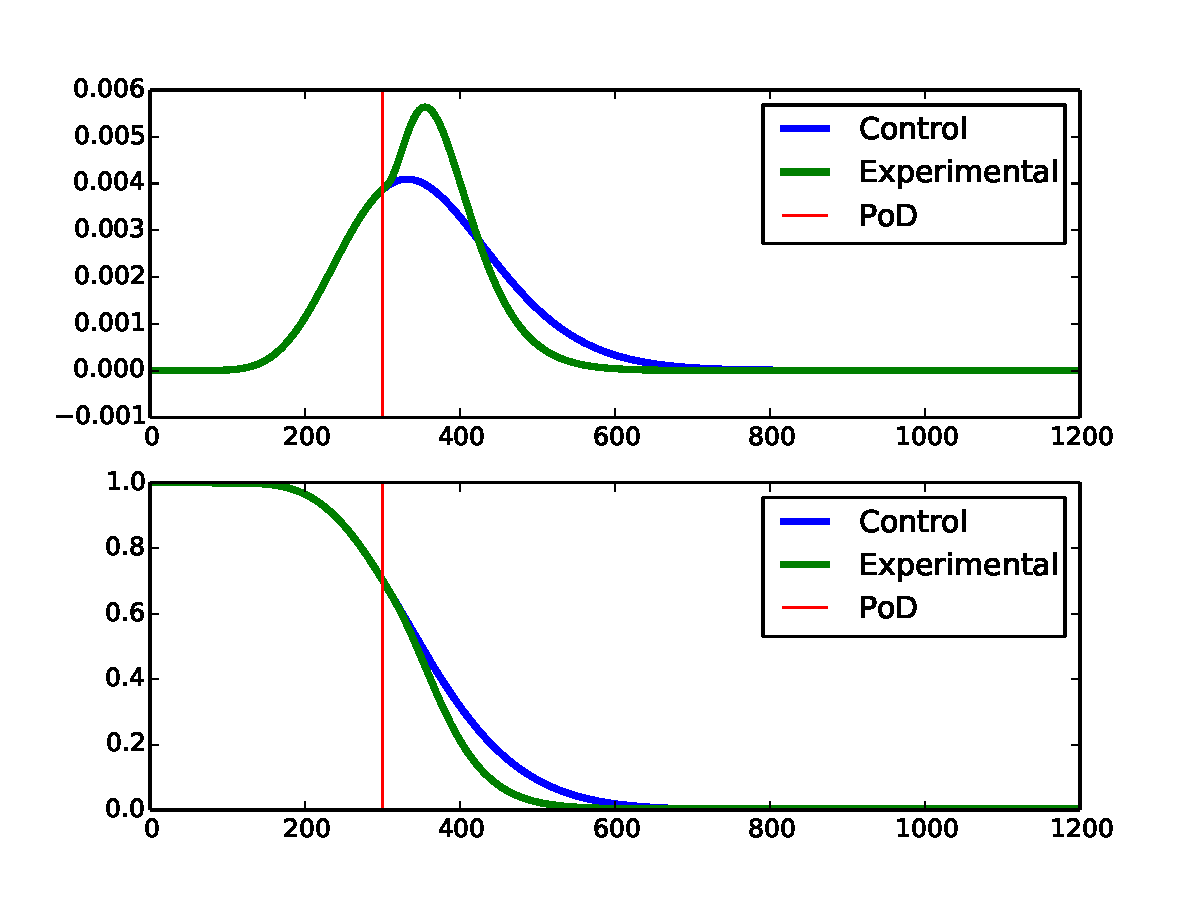
\includegraphics[width=.6\textwidth]{pod.pdf}
 \caption{PDFs (upper panel) and survival functions (lower panel) of the response latencies under 
 control condition (blue lines) and experimental condition (green lines).  The divergence point of 
 the two response-latency distributions is shown as the red vertical lines. \label{fig:pod}}
\end{figure}

Figure \ref{fig:pod} shows the plots generated from the code above. The blue lines show the PDF
(upper panel) and survival function (1-CDF, lower panel) of the response latency under control
condition. Being a convolution of two Gamma distributions, it is an analytic function on the
interval $(0,\infty)$. The green lines show the PDF and survival function of the response latency
under control condition. As the distribution of $X_2$ is not analytic on the complete interval
$(0,\infty)$ (discontinuity at $T=300$ ms), a divergence point may exist at $T=300$ (red vertical
lines).  In fact, that point is visible in both the PDF and the survival function. Hence, this simple
model is able to produce a divergence point as both response-latency distributions are identical
on the interval $[0,300)$ and diverge thereafter.
